\section{CSS3}

CSS3 es la versión más reciente de CSS, compatible con versiones anteriores del mismo, las características nuevas más significantes son el poder aplicar un radio e imagen a los bordes de elementos, varios fondos, animaciones y efectos.


\subsection{Prefijos del proveedor o buscador}

Los \textbf{prefijos del proveedor} (\textbf{o del buscador}) son instrucciones utilizadas para aplicar una propiedad a un buscador que no soporta dicha propiedad, por ejemplo, puede que Safari no soporte la propiedad \textit{border-radious}, por lo que hay que establecer el prefijo de Safari, seguido de la propiedad que deseamos utilizar en el sitio web, con esto, ya podremos trabajar con el radio de bordes de elementos. Los prefijos de algunos buscadores son:
\begin{itemize}
    \item \textbf{-webkit-}: prefijo para Safari, Chrome y buscadores que utilizan el motor \textit{Webkit} (iOS y Android).
    \item \textbf{-moz-}: prefijo para Firefox y buscadores que utilizan el motor de búsqueda de este.
    \item \textbf{-o-}: prefijo para Opera.
    \item \textbf{-ms-}: prefijo para Internet Explorer y Edge.
\end{itemize}

La sintaxis es la siguiente:
\begin{center}
    \textit{
        -webkit-border-radious: 8px; \\
        -o-border-radious: 8px; \\
        -moz-border-radious: 8px; \\
        -ms-border-radious: 8px; \\
    }
\end{center}

\textit{Nota}: actualmente, muchos buscadores ya integran todas las propiedades y características de CSS3, sin embargo, es recomendable conocer estos prefijos para tener una noción de que algunas propiedades tal vez no estén disponibles en el buscador donde estamos desarrollando un proyecto.


\subsection{Esquinas redondeadas}

La propiedad \textbf{border-radius} de CSS permite redondear todas las esquinas de un elemento. Podemos asignar un radio distinto por cada esquina con las propiedades \textbf{border-top-left-radius, border-top-right-radius, border-bottom-right-radius, border-bottom-left-radius}; esta propiedad cuenta con un acceso directo, para evitar escribir todas las propiedades anteriormente mencionadas una por una, como vemos en el siguiente ejemplo y su resultado en la \textit{Figura \ref{fig: 33}}:
\begin{lstlisting}
estilos.css
    /* Redondea todas las esquinas del contenedor en una sola instrucción. */
    .todo-redondeado {
        display: inherit;
        background-color: green;
        color: white;
        padding: 50px;
        margin-bottom: 5px;
        border-radius: 20px;
    }
    /* Redondea algunas esquinas del contenedor en varias instrucciones. */
    .separado-redondeado {
        display: inherit;
        background-color: green;
        color: white;
        padding: 50px;
        margin-bottom: 5px;
        border-top-right-radius: 10px;
        border-bottom-left-radius: 15px;
    }
    /* Redondea todas las esquinas del contenedor en varias instrucciones. */
    .todo-sep-redo {
        display: inherit;
        background-color: green;
        color: white;
        padding: 50px;
        margin-bottom: 5px;
        border-radius: 5px 7px 9px 11px;
    }
    .redondeado {
        display: block;
    }

prueba.html
    <div class="redondeado">
        <div class="todo-redondeado"></div>
        <div class="separado-redondeado"></div>
        <div class="todo-sep-redo"></div>
    </div>
\end{lstlisting}
\begin{figure}[H]
    \centering
    \caption{Diferencia entre valores de propiedad \textit{border-radious}}
    \label{fig: 33}
    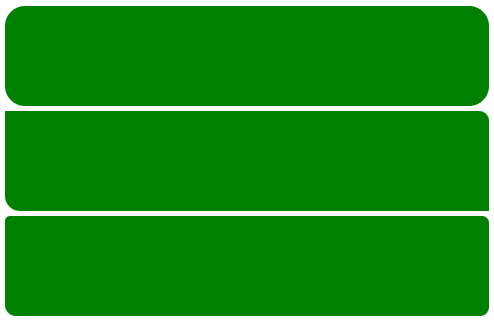
\includegraphics[width=8cm]{ss/border-radious.png}
\end{figure}

Como podemos ver, los valores que acepta esta propiedad son \textbf{Longitudes} (\%, px, pt, cm, em, etc.).


\subsection{Sombras}

La propiedad \textbf{box-shadow} de CSS permite agregar sombra a un elemento HTML. La forma en la que esta sombra es procesada por el buscador mediante los valores aceptados es la siguiente: el primer valor es el \textbf{largo de la sombra sobre el eje horizontal} del elemento, el segundo valor es el \textbf{largo de la sombra en el eje vertical} del elemento y el tercer valor es el \textbf{color de la sombra} (opcional). Además a estos valores, podemos agregar dos valores más: el \textbf{difuminado} y \textbf{propagación de la sombra} (\textit{blur} y \textit{spread}), como su nombre lo indica, modifican el difuminado de la sombra, y cómo esta se propaga alrededor del elemento. Veamos dos ejemplos, el primero sin difuminado ni propagación, el segundo si lo tiene, el resultado está en la \textit{Figura \ref{fig: 34}}:
\begin{lstlisting}
estilos.css
    /* Agrega sombra sin difuminar. */
    .bs1 {
        width: 300px;
        height: 100px;
        background-color: aquamarine;
        box-shadow: 10px 10px #152;
        margin-bottom: 20px;
    }
    /* Agrega sombra difuminada. */
    .bs2 {
        width: 300px;
        height: 100px;
        background-color:blue;
        box-shadow: 10px 10px 5px 5px #878787;
    }

pruebas.html
    <div class="redondeado">
        <div class="bs1"></div>
        <div class="bs2"></div>
    </div>
\end{lstlisting}
\begin{figure}[H]
    \centering
    \caption{Diferencia entre valores de propiedad \textit{box-shadow}}
    \label{fig: 34}
    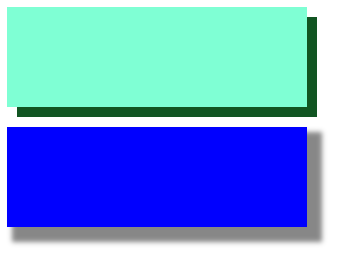
\includegraphics[width=8cm]{ss/box-shadow1.png}
\end{figure}

\textit{Nota}: asignar valores negativos a la propiedad ocasionará que la sombra se posicione en la esquina superior izquierda, no en la esquina inferior derecha.


\subsubsection{Técnicas para el sombreado}

Anteriormente vimos como crear una sombra para un elemento, pero solamente una, esta pudiendo tener su origen en dos ubicaciones distintas fuera del elemento, con la palabra reservada \textbf{inset} podemos crear una sombra dentro del elemento: esta palabra reservada va enseguida del nombre de la propiedad, y podemos asignarle valores como vimos en el tema anterior. Veamos la instrucción:
\begin{center}
    \textit{box-shadow: inset 10px 10px 5px \#888888;}
\end{center}

Esta instrucción creará una sombra interior ubicada en la esquina superior izquierda. Si queremos poner más sombras a un elemento, las podemos separar con una coma (,), como se ve en el siguiente ejemplo y resultado en la \textit{Figura \ref{fig: 35}}
\begin{lstlisting}
estilos.css
    /* Agrega una sombra interna sin difuminar. */
    .bs1 {
        width: 300px;
        height: 100px;
        background-color: aquamarine;
        box-shadow: inset 10px 10px #152;
        margin-bottom: 20px;
    }
    /* Agrega una sombra interna completa semi difuminada. */
    .bs2 {
        width: 300px;
        height: 100px;
        background-color:blue;
        box-shadow: 
        inset 10px 10px 5px 5px #878787,
        inset -10px -10px 5px 5px #878787;
        margin-bottom: 50px;
    }
    /* Agrega varias sombras externas completas difuminadas. */
    .bs3 {
        width: 300px;
        height: 100px;
        background-color:blue;
        box-shadow: 
        0 0 10px 4px #ff6347,
        0 0 10px 30px #ffdab9,
        30px 0 20px 30px #b0e0e6;
        margin-bottom: 20px;
        margin-left: 35px;
    }

prueba.html
    <div class="bs1"></div>
    <div class="bs2"></div>
    <div class="bs3"></div>
\end{lstlisting}
\begin{figure}[H]
    \centering
    \caption{Diferencia entre valores de propiedad \textit{box-shadow}}
    \label{fig: 35}
    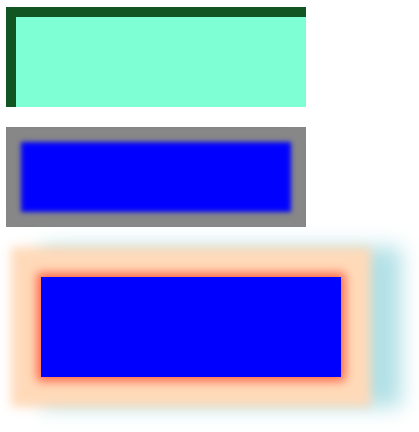
\includegraphics[width=8cm]{ss/box-shadow2.png}
\end{figure}

Como podemos ver, el primer rectángulo solo tiene una sombra interna, el segundo posee dos sombras internas, y el tercero posee tres sombras externas, una encima de otra, siguiendo el orden del código mostrado. Nótese que no existe una palabra reservada para sombras externas.


\subsubsection{Sombras en texto}

La propiedad \textbf{text-shadow} permite agregar una sombra al texto de un objeto o etiqueta HTML. Cuenta con cuatro valores: sombra horizontal, sombra vertical, difuminado y color; las sombras horizontal y vertical posiciona la sombra por debajo del texto en dichos ejes, podemos hacer que la sombra sea completamente definida o difuminada, y por último, podemos darle un color. Los primeros tres valores aceptan \textit{Longitudes} (\%, px, pt, cm, em, etc. También el valor \textit{none} para no asignar alguna sombra al texto), mientras que el último valor acepta valores de las distintas \textit{Herramientas de colores} con las que cuenta CSS.

Al igual que con \textit{box-shadow}, podemos crear varias sombras en el texto (inclusive negativas), veamos un ejemplo y su resultado en la \textit{Figura \ref{fig: 36}}:
\begin{lstlisting}
estilos.css
    /* Agrega una sombra. */
    .s1 {
        text-shadow: 3px 3px 2px #152;
        margin-bottom: 20px;
    }
    /* Agrega dos sombras. */
    .s2 {
        text-shadow: 
        10px 10px 5px #878787,
        -10px -10px 5px #900000;
        margin-bottom: 50px;
    }

prueba.html
    <p class="s1">Sombra 1</p>
    <p class="s2">Sombra 2</p>
\end{lstlisting}
\begin{figure}[H]
    \centering
    \caption{Diferencia entre valores de propiedad \textit{text-shadow}}
    \label{fig: 36}
    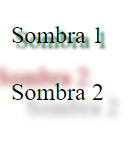
\includegraphics[width=3cm]{ss/text-shadow.png}
\end{figure}

Solo recuerde que las sombras se ven más realistas si:
\begin{itemize}
    \item una sombra cercana no está tan difuminada,
    \item una soma lejana si está más difuminada
\end{itemize}


\subsection{Transparencia}

Previo a CSS3, para lograr que un elemento tuviera transparencia, se utiliza la propiedad \textit{background-image} con una imagen en formato PNG, ahora, hay otros métodos para lograr este cometido. Con esta versión de CSS, se soporta ahora nombres de colores, hexadecimales, RGB y dos nuevas herramientas, que la \textit{Tabla \ref{tab: 4}} muestra:
\begin{table}[H]
    \centering
    \caption{Nuevas herramientas para colores en CSS3}
    \label{tab: 4}
    \begin{tabular}{m{3cm} m{8cm} m{4cm}}
        \hline
        \textbf{Herramienta} & \textbf{Definición} & \textbf{Ejemplo} \\
        \hline
        \parbox{3cm}{Colores RGBA}    & \parbox{8cm}{Extensión de los colores RGB con un valor \textbf{alfa}, el cual especifica la opacidad del color} & \parbox{4cm}{ rgba(204, 29, 29, 1.0); } \\
        \hline
        \parbox{3cm}{Colores HSL}     & \parbox{8cm}{Colores \textbf{Hue, Saturation, Lightness} (Matiz o color, Saturación, Luminosidad o claridad), es otra forma de expresar colores: el primero representa el color (los valores van de 0  360, donde 0 y 360 es rojo, 120 es verde y 240 es azul, en base a esto, se juega con estos valores para obtener el color deseado), el segundo la saturación (se mide en porcentajes, 100\% es el color completo y como tal) y el tercero la claridad del color (0\% es oscuro o negro, 100\% es blanco)} & \parbox{4cm}{ hsl(0, 10\%, 60\%); } \\
        \hline
        \parbox{3cm}{Colores HSLA}    & \parbox{8cm}{Extensión de los colores HSL con un valor \textbf{alfa}, el cual especifica la opacidad del color} & \parbox{4cm}{ hsla(147, 50\%,\\ 47\%, 0.5); } \\
        \hline
    \end{tabular}
\end{table}

Veamos el resultado de los ejemplos anteriores en la \textit{Figura \ref{fig: 37}}:
\begin{lstlisting}
estilos.css
    /* Establece color con RGBA y sin transparencia (1.0). */
    #rgba1 {
        width: 100px;
        height: 100px;
        background-color: rgba(204, 29, 29, 1.0);
        margin-bottom: 10px;
    }
    /* Establece color con RGBA y con transparencia de 0.1. */
    #rgba2 {
        width: 100px;
        height: 100px;
        background-color: rgba(161, 30, 30, 0.1);
        margin-bottom: 10px;
    }
    /* Establece color con HSL y con transparencia del 60%. */
    #hsl1 {
        width: 100px;
        height: 100px;
        background-color: hsl(0, 10%, 60%);
        margin-bottom: 10px;
    }
    /* Establece color con HSLA y con transparencia de 0.5. */
    #hsl2 {
        width: 100px;
        height: 100px;
        background-color: hsla(147, 50%, 47%, 0.5);
    }

prueba.html
    <div id="rgba1"></div>
    <div id="rgba2"></div>
    <div id="hsl1"></div>
    <div id="hsl2"></div>
\end{lstlisting}
\begin{figure}[H]
    \centering
    \caption{Uso de RGBA, HSL y HSLA}
    \label{fig: 37}
    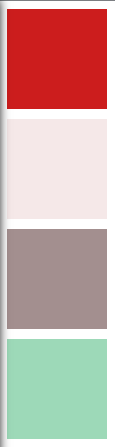
\includegraphics[height=9cm]{ss/rgba,hsl,hsla.png}
\end{figure}


\subsection{Pseudo clases}

Bien vimos que, para estilizar un elemento específico, le asignamos un Id o Clase, y dicha Clase o Id, se le aplican instrucciones CSS. En caso de que se tengan múltiples etiquetas dentro de otra, cada una de ellas debería tener una Clase o Id para ser modificadas por separado.

Es aquí donde entran las \textbf{Pseudo clases}, estas permiten modificar un elemento sin tener que asignarle una Clase o Id ni utilizar JavaScript. Existen muchas Pseudo clases, para estos apuntes, hablaremos de \textit{:first-child} y \textit{:last-child}:
\begin{itemize}
    \item \textbf{:first-child}: aplica un estilo al primer elemento dentro de otro.
    \item \textbf{:last-child}: aplica un estilo al último elemento dentro de otro.
\end{itemize}

Veamos un ejemplo y su resultado en la \textit{Figura \ref{fig: 38}}:
\begin{lstlisting}
estilos.css
    /* Clase padre con color de texto rojo. */
    .pseudo {
    color: red;
    }
    /* Cambia el color de texto del primer hijo de la clase padre. */
    .pseudo p:first-child {
        color: blue;
    }
    /* Cambia el color de texto del último hijo de la clase padre. */
    .pseudo p:last-child {
        color: violet;
    }

prueba.html
    <div class="pseudo">
        <p>Este es el primer párrafo.</p>
        <p>Este es el segundo párrafo.</p>
        <p>Este es el tercer párrafo.</p>
        <p>Este es el cuarto párrafo.</p>
        <p>Este es el quinto párrafo.</p>
        <p>Este es el sexto párrafo.</p>
    </div>
\end{lstlisting}
\begin{figure}[H]
    \centering
    \caption{Uso de las Pseudo clases}
    \label{fig: 38}
    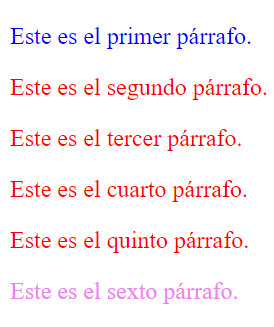
\includegraphics[height=5cm]{ss/pseudo-clases.png}
\end{figure}

Estas dos Pseudo clases son de las más utilizadas, pero existen más, te invito a investigar qué utilidad tienen el resto de Pseudo clases disponibles.


\subsection{Pseudo elementos}

Otra gran utilidad de estas Pseudo herramientas disponibles en CSS son los \textbf{Pseudo elementos}, estos permiten estilizar una parte o elemento de una etiqueta HTML. Las Pseudo clases utilizan los \textit{dos puntos} (:), los Pseudo elementos utilizan \textit{doble dos puntos} (::) para ser trabajados. Los cinco Pseudo elementos más utilizados son:
\begin{itemize}
    \item \textbf{::first-line}: selecciona la primer línea de un texto en una etiqueta.
    \item \textbf{::first-letter}: selecciona la primer letra de un texto o palabra en una etiqueta.
    \item \textbf{::selection}: toma el texto seleccionado de una etiqueta por el usuario
    \item \textbf{::before}: inserta un contenido antes de una etiqueta.
    \item \textbf{::after}: inserta un contenido después de una etiqueta.
\end{itemize}

Algunos de estos Pseudo elementos no están disponibles en ciertos navegadores, por lo que tendrá que acudir a los \textbf{prefijos de buscadores}. Veamos un ejemplo de estos Pseudo elementos y su resultado en la \textit{Figura \ref{fig: 39}}:
\begin{lstlisting}
estilos.css
    /* Cambia el color de la primer letra. */
    p::first-letter {
        color: blue;
    }
    /* Cambia el color de la primer línea del texto. */
    p::first-line {
        color: red;
    }
    /* Cambia el color del texto seleccionado. */
    p::selection {
        background-color: green;
        color:white;
    }
    /* Agrega algo antes de un elemento. */
    p::before {
        content: url(bola.png);
    }
    /* Agrega algo después de un elemento. */
    p::after {
        content: url(bola.png);
    }

prueba.html
    <div class="pseudo">
        <p>Lorem ipsum dolor sit amet consectetur adipisicing elit. Assumenda distinctio ullam delectus porro odit sequi aperiam, amet commodi molestias beatae veniam obcaecati similique sint nulla, consequuntur veritatis, magni autem est.</p>
        <p>Lorem ipsum dolor sit amet consectetur adipisicing elit. Assumenda distinctio ullam delectus porro odit sequi aperiam, amet commodi molestias beatae veniam obcaecati similique sint nulla, consequuntur veritatis, magni autem est.</p>
        <p>Lorem ipsum dolor sit amet consectetur adipisicing elit. Assumenda distinctio ullam delectus porro odit sequi aperiam, amet commodi molestias beatae veniam obcaecati similique sint nulla, consequuntur veritatis, magni autem est.</p>
        <p>Lorem ipsum dolor sit amet consectetur adipisicing elit. Assumenda distinctio ullam delectus porro odit sequi aperiam, amet commodi molestias beatae veniam obcaecati similique sint nulla, consequuntur veritatis, magni autem est.</p>
        <p>Lorem ipsum dolor sit amet consectetur adipisicing elit. Assumenda distinctio ullam delectus porro odit sequi aperiam, amet commodi molestias beatae veniam obcaecati similique sint nulla, consequuntur veritatis, magni autem est.</p>
    </div>
\end{lstlisting}
\begin{figure}[H]
    \centering
    \caption{Uso de los Pseudo elementos}
    \label{fig: 39}
    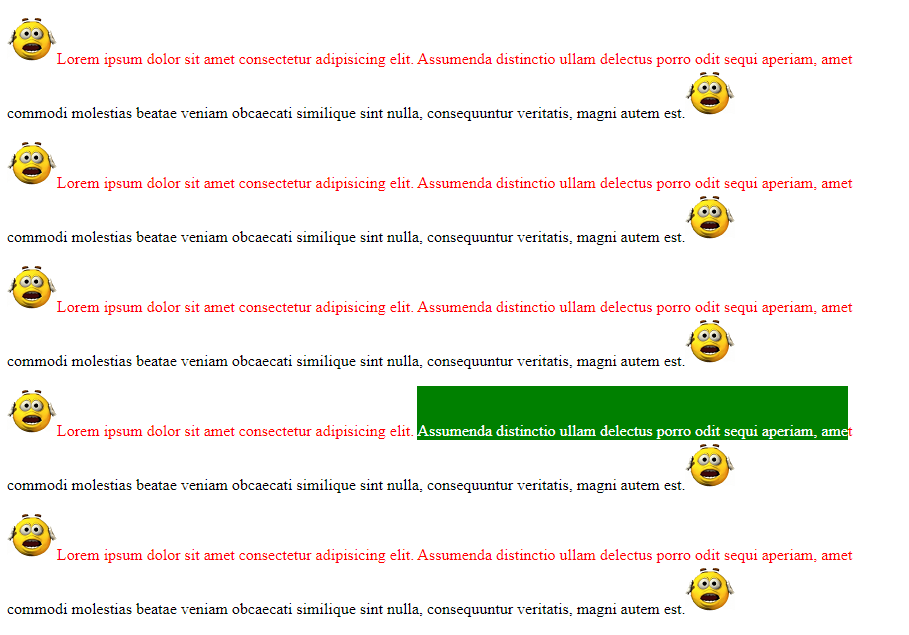
\includegraphics[width=12cm]{ss/pseudo-elementos.png}
\end{figure}

En el caso de \textit{first-letter} esta se ve sobre escrita por \textit{first-line}, por lo cual no se aprecia en la figura anterior. Al igual que con las Pseudo clases, se le invita a investigar más Pseudo elementos existentes.


\subsection{word-wrap}
\
La propiedad \textbf{word-wrap} de CSS permite establecer si una palabra da un salto de línea cuando topa con el límite de su etiqueta o contenedor; los valores permitidos son:
\begin{itemize}
    \item \textbf{normal}: el texto mantiene su largo.
    \item \textbf{break-word}: el texto da un salto de línea.
    \item \textbf{inherit}, \textbf{initial} y \textbf{unset}.
\end{itemize}

Veamos un ejemplo claro de esta propiedad y su resultado en la \textit{Figura \ref{fig: 40}}:
\begin{lstlisting}
estilos.css
    /* Clase que no da salto de línea. */
    .wwn {
        width: 200px;
        height: 100px;
        border: 2px solid black;
        word-wrap: normal;
    }
    /* Clase que no da salto de línea. */
    .wwww {
        width: 200px;
        height: 100px;
        border: 2px solid black;
        word-wrap: break-word;
    }

prueba.html
    <p class="wwn">Esta caja tiene una palabra muy larga: njfsadfnjiaifiafiaisiajfisjadifisadnfsiadfnjisdjfjiasdfjisadfidanjinj</p>
    <p class="wwww">Esta caja tiene una palabra muy larga: njfsadfnjiaifiafiaisiajfisjadifisadnfsiadfnjisdjfjiasdfjisadfidanjinj</p>
\end{lstlisting}
\begin{figure}[H]
    \centering
    \caption{Diferencia entre valores de propiedad \textit{word-wrap}}
    \label{fig: 40}
    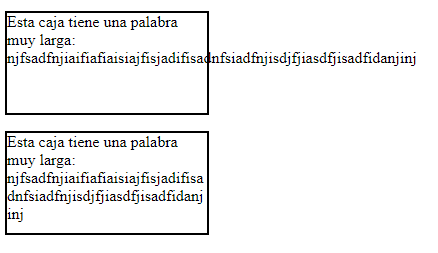
\includegraphics[width=10cm]{ss/word-wrap.png}
\end{figure}


\subsection{@font-face}

La regla \textbf{@font-face} permite descargar u obtener una fuente o tipo de letra de un servidor y establecerla en todo nuestro sitio web, de esta manera, las fuentes disponibles en el sitio ya no están limitadas en las que están instaladas en la máquina del usuario que accede al sitio.

Esta regla trabaja con los formatos \textbf{Embedded OpenType} (eot), \textbf{True Type Fonts} (ttf) y \textbf{OpenType Fonts} (otf), los siguientes navegadores aceptan los formatos mencionados:
\begin{itemize}
    \item Firefox, Safari, Chrome y Opera: .ttf y .otf.
    \item Internet Explorer: .eot
\end{itemize}

Para utilizar esta regla, debe escribir el nombre de la regla (@font-face), abrir llaves, darle un nombre a la fuente, la ruta donde está almacenada la fuente y alguna personalización extra, como se ve a continuación:
\begin{lstlisting}
estilos.css
    /* Define dos reglas iguales pero con distinto estilo. */
    @font-face {
      font-family: Delicious; 
      src: url('Delicious-Roman.otf'); 
    } 
    @font-face { 
      font-family: Delicious; 
      font-weight: bold; 
      src: url('Delicious-Bold.otf'); 
    }
    /* Asigna las reglas a las etiquetas "h1". */
    h1 {
       font-family: Delicious, sans-serif; 
    }

prueba.html
    <h1>Hola mundo</h1>
\end{lstlisting}

En caso de que queramos que todo el sitio tenga la nueva fuente, en vez de asignarla a la etiqueta "h1", se la asignamos a "body."

Las fuentes más utilizadas actualmente son las de Google, esto debido a que es por este buscador que los usuarios se conectan a Internet y realizan sus búsquedas, por lo que es bueno utilizar dichas fuentes para cargar nuestro sitio web, puede ver todas las fuentes disponibles en este \href{https://fonts.google.com/}{enlace} (aunque tiene una distinta implementación).

Puede buscar fuentes con los formatos anteriormente mencionados en Internet y aplicarlas al sitio web, como se ve en el ejemplo siguiente y su resultado en la \textit{Figura \ref{fig: 41}}:
\begin{lstlisting}
estilos.css
    /* Asigna la fuente importada a las etiquetas "h1". */
    h1 {
        font-family: 'Open Sans', sans-serif;
    }
    
prueba.html
    <h1>Hola mundo</h1>
\end{lstlisting}
\begin{figure}[H]
    \centering
    \caption{Uso de la regla \textit{@font-face}}
    \label{fig: 41}
    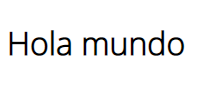
\includegraphics[width=3cm]{ss/font-face.png}
\end{figure}
